% Created by tikzDevice version 0.12.6 on 2025-10-11 22:33:34
% !TEX encoding = UTF-8 Unicode
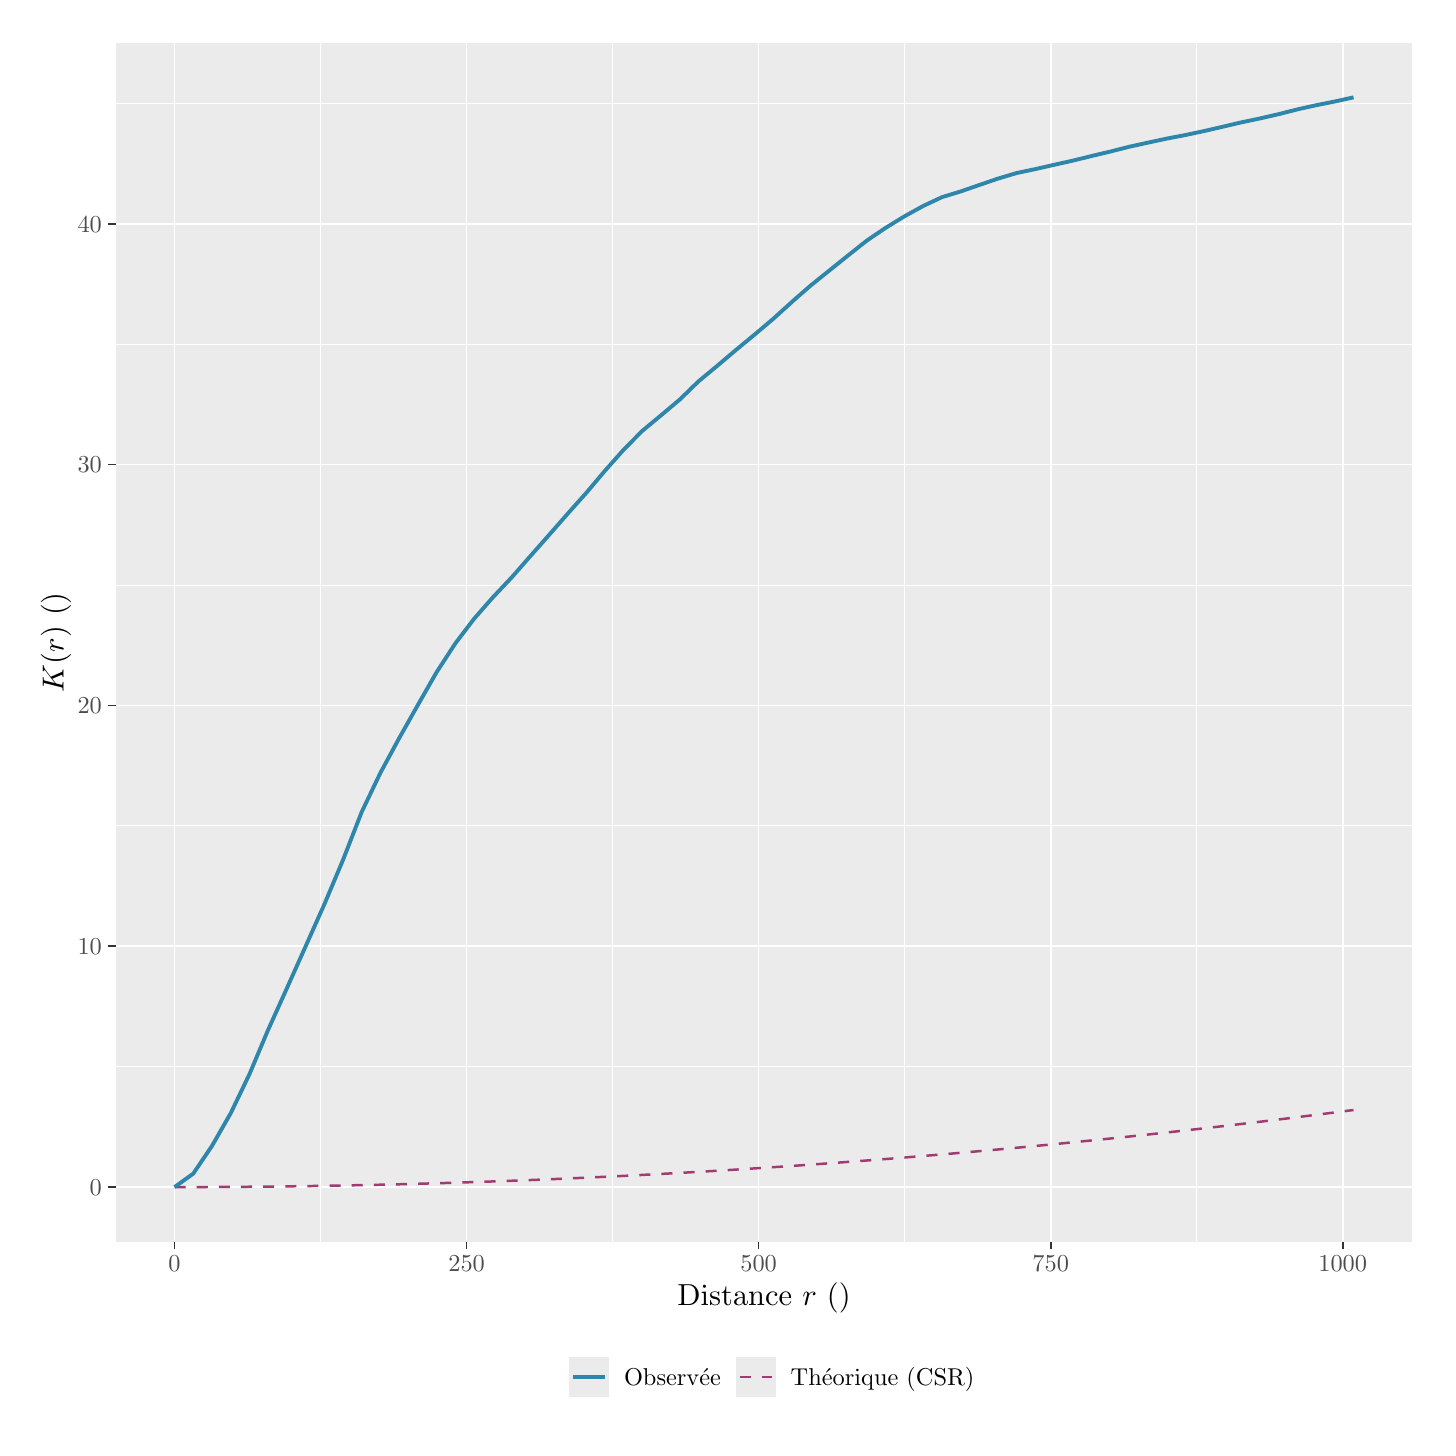
\begin{tikzpicture}[x=1pt,y=1pt]
\definecolor{fillColor}{RGB}{255,255,255}
\path[use as bounding box,fill=fillColor,fill opacity=0.00] (0,0) rectangle (505.89,505.89);
\begin{scope}
\path[clip] (  0.00,  0.00) rectangle (505.89,505.89);
\definecolor{drawColor}{RGB}{255,255,255}
\definecolor{fillColor}{RGB}{255,255,255}

\path[draw=drawColor,line width= 0.6pt,line join=round,line cap=round,fill=fillColor] (  0.00,  0.00) rectangle (505.89,505.89);
\end{scope}
\begin{scope}
\path[clip] ( 31.78, 67.26) rectangle (500.39,500.39);
\definecolor{fillColor}{gray}{0.92}

\path[fill=fillColor] ( 31.78, 67.26) rectangle (500.39,500.39);
\definecolor{drawColor}{RGB}{255,255,255}

\path[draw=drawColor,line width= 0.3pt,line join=round] ( 31.78,130.45) --
	(500.39,130.45);

\path[draw=drawColor,line width= 0.3pt,line join=round] ( 31.78,217.47) --
	(500.39,217.47);

\path[draw=drawColor,line width= 0.3pt,line join=round] ( 31.78,304.48) --
	(500.39,304.48);

\path[draw=drawColor,line width= 0.3pt,line join=round] ( 31.78,391.50) --
	(500.39,391.50);

\path[draw=drawColor,line width= 0.3pt,line join=round] ( 31.78,478.52) --
	(500.39,478.52);

\path[draw=drawColor,line width= 0.3pt,line join=round] (105.84, 67.26) --
	(105.84,500.39);

\path[draw=drawColor,line width= 0.3pt,line join=round] (211.37, 67.26) --
	(211.37,500.39);

\path[draw=drawColor,line width= 0.3pt,line join=round] (316.90, 67.26) --
	(316.90,500.39);

\path[draw=drawColor,line width= 0.3pt,line join=round] (422.43, 67.26) --
	(422.43,500.39);

\path[draw=drawColor,line width= 0.6pt,line join=round] ( 31.78, 86.94) --
	(500.39, 86.94);

\path[draw=drawColor,line width= 0.6pt,line join=round] ( 31.78,173.96) --
	(500.39,173.96);

\path[draw=drawColor,line width= 0.6pt,line join=round] ( 31.78,260.98) --
	(500.39,260.98);

\path[draw=drawColor,line width= 0.6pt,line join=round] ( 31.78,347.99) --
	(500.39,347.99);

\path[draw=drawColor,line width= 0.6pt,line join=round] ( 31.78,435.01) --
	(500.39,435.01);

\path[draw=drawColor,line width= 0.6pt,line join=round] ( 53.08, 67.26) --
	( 53.08,500.39);

\path[draw=drawColor,line width= 0.6pt,line join=round] (158.61, 67.26) --
	(158.61,500.39);

\path[draw=drawColor,line width= 0.6pt,line join=round] (264.14, 67.26) --
	(264.14,500.39);

\path[draw=drawColor,line width= 0.6pt,line join=round] (369.66, 67.26) --
	(369.66,500.39);

\path[draw=drawColor,line width= 0.6pt,line join=round] (475.19, 67.26) --
	(475.19,500.39);
\definecolor{drawColor}{RGB}{162,59,114}

\path[draw=drawColor,line width= 0.9pt,dash pattern=on 4pt off 4pt ,line join=round] ( 53.08, 86.94) --
	( 59.84, 86.95) --
	( 66.60, 86.97) --
	( 73.37, 87.01) --
	( 80.13, 87.06) --
	( 86.89, 87.12) --
	( 93.65, 87.20) --
	(100.41, 87.29) --
	(107.18, 87.39) --
	(113.94, 87.51) --
	(120.70, 87.65) --
	(127.46, 87.79) --
	(134.22, 87.95) --
	(140.99, 88.13) --
	(147.75, 88.32) --
	(154.51, 88.52) --
	(161.27, 88.74) --
	(168.03, 88.97) --
	(174.80, 89.22) --
	(181.56, 89.48) --
	(188.32, 89.75) --
	(195.08, 90.04) --
	(201.84, 90.34) --
	(208.61, 90.66) --
	(215.37, 90.98) --
	(222.13, 91.33) --
	(228.89, 91.69) --
	(235.66, 92.06) --
	(242.42, 92.44) --
	(249.18, 92.84) --
	(255.94, 93.26) --
	(262.70, 93.69) --
	(269.47, 94.13) --
	(276.23, 94.58) --
	(282.99, 95.05) --
	(289.75, 95.54) --
	(296.51, 96.04) --
	(303.28, 96.55) --
	(310.04, 97.07) --
	(316.80, 97.61) --
	(323.56, 98.17) --
	(330.32, 98.74) --
	(337.09, 99.32) --
	(343.85, 99.92) --
	(350.61,100.53) --
	(357.37,101.15) --
	(364.13,101.79) --
	(370.90,102.44) --
	(377.66,103.11) --
	(384.42,103.79) --
	(391.18,104.48) --
	(397.94,105.19) --
	(404.71,105.91) --
	(411.47,106.65) --
	(418.23,107.40) --
	(424.99,108.17) --
	(431.76,108.94) --
	(438.52,109.74) --
	(445.28,110.54) --
	(452.04,111.36) --
	(458.80,112.20) --
	(465.57,113.05) --
	(472.33,113.91) --
	(479.09,114.79);
\definecolor{drawColor}{RGB}{46,134,171}

\path[draw=drawColor,line width= 1.4pt,line join=round] ( 53.08, 86.94) --
	( 59.84, 91.80) --
	( 66.60,101.81) --
	( 73.37,113.63) --
	( 80.13,127.71) --
	( 86.89,143.77) --
	( 93.65,158.74) --
	(100.41,173.88) --
	(107.18,189.06) --
	(113.94,205.14) --
	(120.70,222.48) --
	(127.46,236.62) --
	(134.22,249.12) --
	(140.99,261.13) --
	(147.75,272.96) --
	(154.51,283.36) --
	(161.27,292.24) --
	(168.03,299.96) --
	(174.80,307.13) --
	(181.56,314.83) --
	(188.32,322.48) --
	(195.08,330.20) --
	(201.84,337.77) --
	(208.61,345.79) --
	(215.37,353.41) --
	(222.13,360.22) --
	(228.89,365.83) --
	(235.66,371.53) --
	(242.42,378.10) --
	(249.18,383.70) --
	(255.94,389.43) --
	(262.70,395.00) --
	(269.47,400.73) --
	(276.23,406.85) --
	(282.99,412.76) --
	(289.75,418.19) --
	(296.51,423.62) --
	(303.28,428.99) --
	(310.04,433.56) --
	(316.80,437.70) --
	(323.56,441.44) --
	(330.32,444.62) --
	(337.09,446.69) --
	(343.85,449.03) --
	(350.61,451.34) --
	(357.37,453.36) --
	(364.13,454.78) --
	(370.90,456.33) --
	(377.66,457.83) --
	(384.42,459.51) --
	(391.18,461.11) --
	(397.94,462.83) --
	(404.71,464.32) --
	(411.47,465.77) --
	(418.23,467.07) --
	(424.99,468.50) --
	(431.76,470.07) --
	(438.52,471.66) --
	(445.28,473.08) --
	(452.04,474.63) --
	(458.80,476.35) --
	(465.57,477.86) --
	(472.33,479.21) --
	(479.09,480.70);
\end{scope}
\begin{scope}
\path[clip] (  0.00,  0.00) rectangle (505.89,505.89);
\definecolor{drawColor}{gray}{0.30}

\node[text=drawColor,anchor=base east,inner sep=0pt, outer sep=0pt, scale=  0.88] at ( 26.83, 83.94) {0};

\node[text=drawColor,anchor=base east,inner sep=0pt, outer sep=0pt, scale=  0.88] at ( 26.83,170.95) {10};

\node[text=drawColor,anchor=base east,inner sep=0pt, outer sep=0pt, scale=  0.88] at ( 26.83,257.97) {20};

\node[text=drawColor,anchor=base east,inner sep=0pt, outer sep=0pt, scale=  0.88] at ( 26.83,344.99) {30};

\node[text=drawColor,anchor=base east,inner sep=0pt, outer sep=0pt, scale=  0.88] at ( 26.83,432.00) {40};
\end{scope}
\begin{scope}
\path[clip] (  0.00,  0.00) rectangle (505.89,505.89);
\definecolor{drawColor}{gray}{0.20}

\path[draw=drawColor,line width= 0.6pt,line join=round] ( 29.03, 86.94) --
	( 31.78, 86.94);

\path[draw=drawColor,line width= 0.6pt,line join=round] ( 29.03,173.96) --
	( 31.78,173.96);

\path[draw=drawColor,line width= 0.6pt,line join=round] ( 29.03,260.98) --
	( 31.78,260.98);

\path[draw=drawColor,line width= 0.6pt,line join=round] ( 29.03,347.99) --
	( 31.78,347.99);

\path[draw=drawColor,line width= 0.6pt,line join=round] ( 29.03,435.01) --
	( 31.78,435.01);
\end{scope}
\begin{scope}
\path[clip] (  0.00,  0.00) rectangle (505.89,505.89);
\definecolor{drawColor}{gray}{0.20}

\path[draw=drawColor,line width= 0.6pt,line join=round] ( 53.08, 64.51) --
	( 53.08, 67.26);

\path[draw=drawColor,line width= 0.6pt,line join=round] (158.61, 64.51) --
	(158.61, 67.26);

\path[draw=drawColor,line width= 0.6pt,line join=round] (264.14, 64.51) --
	(264.14, 67.26);

\path[draw=drawColor,line width= 0.6pt,line join=round] (369.66, 64.51) --
	(369.66, 67.26);

\path[draw=drawColor,line width= 0.6pt,line join=round] (475.19, 64.51) --
	(475.19, 67.26);
\end{scope}
\begin{scope}
\path[clip] (  0.00,  0.00) rectangle (505.89,505.89);
\definecolor{drawColor}{gray}{0.30}

\node[text=drawColor,anchor=base,inner sep=0pt, outer sep=0pt, scale=  0.88] at ( 53.08, 56.30) {0};

\node[text=drawColor,anchor=base,inner sep=0pt, outer sep=0pt, scale=  0.88] at (158.61, 56.30) {250};

\node[text=drawColor,anchor=base,inner sep=0pt, outer sep=0pt, scale=  0.88] at (264.14, 56.30) {500};

\node[text=drawColor,anchor=base,inner sep=0pt, outer sep=0pt, scale=  0.88] at (369.66, 56.30) {750};

\node[text=drawColor,anchor=base,inner sep=0pt, outer sep=0pt, scale=  0.88] at (475.19, 56.30) {1000};
\end{scope}
\begin{scope}
\path[clip] (  0.00,  0.00) rectangle (505.89,505.89);
\definecolor{drawColor}{RGB}{0,0,0}

\node[text=drawColor,anchor=base,inner sep=0pt, outer sep=0pt, scale=  1.10] at (266.08, 44.22) {Distance $r$ (\unit{\m})};
\end{scope}
\begin{scope}
\path[clip] (  0.00,  0.00) rectangle (505.89,505.89);
\definecolor{drawColor}{RGB}{0,0,0}

\node[text=drawColor,rotate= 90.00,anchor=base,inner sep=0pt, outer sep=0pt, scale=  1.10] at ( 13.01,283.82) {$K(r)$ (\unit{\km\squared})};
\end{scope}
\begin{scope}
\path[clip] (  0.00,  0.00) rectangle (505.89,505.89);
\definecolor{fillColor}{RGB}{255,255,255}

\path[fill=fillColor] (184.54,  5.50) rectangle (347.63, 30.95);
\end{scope}
\begin{scope}
\path[clip] (  0.00,  0.00) rectangle (505.89,505.89);
\definecolor{fillColor}{gray}{0.92}

\path[fill=fillColor] (195.54, 11.00) rectangle (210.00, 25.45);
\definecolor{drawColor}{RGB}{46,134,171}

\path[draw=drawColor,line width= 1.4pt,line join=round] (196.99, 18.23) -- (208.55, 18.23);
\end{scope}
\begin{scope}
\path[clip] (  0.00,  0.00) rectangle (505.89,505.89);
\definecolor{fillColor}{gray}{0.92}

\path[fill=fillColor] (255.78, 11.00) rectangle (270.23, 25.45);
\definecolor{drawColor}{RGB}{162,59,114}

\path[draw=drawColor,line width= 0.9pt,dash pattern=on 4pt off 4pt ,line join=round] (257.22, 18.23) -- (268.78, 18.23);
\end{scope}
\begin{scope}
\path[clip] (  0.00,  0.00) rectangle (505.89,505.89);
\definecolor{drawColor}{RGB}{0,0,0}

\node[text=drawColor,anchor=base west,inner sep=0pt, outer sep=0pt, scale=  0.88] at (215.50, 15.22) {Observée};
\end{scope}
\begin{scope}
\path[clip] (  0.00,  0.00) rectangle (505.89,505.89);
\definecolor{drawColor}{RGB}{0,0,0}

\node[text=drawColor,anchor=base west,inner sep=0pt, outer sep=0pt, scale=  0.88] at (275.73, 15.22) {Théorique (CSR)};
\end{scope}
\end{tikzpicture}
